\documentclass[10pt,a4paper]{article}
\usepackage[T1]{fontenc}
\usepackage[utf8]{inputenc}
\usepackage[french]{babel}
\usepackage[oldstylenums]{kpfonts}
\usepackage{microtype}
\usepackage{amsmath,amssymb}
\usepackage[margin=2.1cm,top=1.9cm,bottom=2.2cm]{geometry}
\usepackage{booktabs}
\usepackage{graphicx}
\usepackage{enumitem}
\usepackage{xcolor}
\usepackage[most]{tcolorbox}
\usepackage{titlesec}
\usepackage{fancyhdr}
\usepackage{hyperref}

% ---------------------------------------------------------------- couleurs
\definecolor{encre}{HTML}{1A2233}
\definecolor{accent}{HTML}{28527A}
\definecolor{okvert}{HTML}{2E7D32}
\definecolor{okvertpale}{HTML}{E8F3E9}
\definecolor{nonrouge}{HTML}{B3402A}
\definecolor{nonrougepale}{HTML}{FBEDE9}
\definecolor{mixte}{HTML}{9A6A00}
\definecolor{mixtepale}{HTML}{FCF4E0}
\definecolor{grisdoux}{HTML}{F2F4F7}

\hypersetup{colorlinks=true,linkcolor=accent,urlcolor=accent}
\color{encre}

% ------------------------------------------------------------------ titres
\titleformat{\section}
  {\Large\bfseries\color{accent}}{\thesection}{0.7em}{}
  [{\color{accent!40}\titlerule[0.6pt]}]
\titleformat{\subsection}
  {\large\bfseries\color{encre}}{\thesubsection}{0.6em}{}
\titlespacing{\section}{0pt}{16pt}{8pt}

% ------------------------------------------------------------------ badges
\newcommand{\badgeOK}[1]{\tcbox[on line, colback=okvertpale, colframe=okvert,
  boxrule=0.6pt, arc=2pt, left=3pt, right=3pt, top=1pt, bottom=1pt]
  {\small\bfseries\color{okvert}#1}}
\newcommand{\badgeNO}[1]{\tcbox[on line, colback=nonrougepale, colframe=nonrouge,
  boxrule=0.6pt, arc=2pt, left=3pt, right=3pt, top=1pt, bottom=1pt]
  {\small\bfseries\color{nonrouge}#1}}
\newcommand{\badgeMI}[1]{\tcbox[on line, colback=mixtepale, colframe=mixte,
  boxrule=0.6pt, arc=2pt, left=3pt, right=3pt, top=1pt, bottom=1pt]
  {\small\bfseries\color{mixte}#1}}

\newtcolorbox{encadre}[2][accent]{enhanced, colback=#1!4, colframe=#1,
  boxrule=0.8pt, arc=3pt, left=8pt, right=8pt, top=6pt, bottom=6pt,
  title={\bfseries #2}, fonttitle=\color{white}}

\newcommand{\NW}{\mathrm{NW}}
\newcommand{\code}[1]{\texttt{#1}}

% ------------------------------------------------------------------ entête
\pagestyle{fancy}
\fancyhf{}
\fancyhead[L]{\small\color{accent}Réplication critique M2 — synthèse finale}
\fancyhead[R]{\small\color{accent}\thepage\,/\,\pageref{LastPage}}
\renewcommand{\headrulewidth}{0.4pt}
\renewcommand{\headrule}{\color{accent!40}\hrule width\headwidth height 0.4pt}
\usepackage{lastpage}

\begin{document}

% =================================================================== bandeau
\begin{tcolorbox}[enhanced, colback=accent, colframe=accent, arc=6pt,
  left=14pt, right=14pt, top=12pt, bottom=12pt]
\color{white}
{\LARGE\bfseries Le modèle M2 à l'épreuve :\\[2pt]
réplication critique et verdicts}\\[8pt]
{\large Distribution Boltzmann--Pareto par auto-organisation critique —
qu'est-ce qui tient vraiment ?}\\[10pt]
\small Agent de réplication (workspace \code{m2\_fable}) \hfill 3 juillet 2026
\end{tcolorbox}

\vspace{6pt}
\noindent
\begin{tcolorbox}[colback=grisdoux, colframe=grisdoux, arc=3pt]
\small\textbf{Dossier} : implémentation propre \code{src/m2/} (37 tests
verts) · $\sim$40 simulations archivées · 5 rapports LaTeX
(\code{reports/01\ldots05}) · journal de recherche · données et JSON de
validation sous \code{experiments/m2/results/}. Ce document est la synthèse
exécutive ; chaque affirmation est traçable dans les rapports détaillés.
\end{tcolorbox}

% ============================================================ verdict global
\section*{Verdict en une phrase}
\begin{encadre}{Le résultat central}
M2 atteint trois de ses quatre cibles phénoménologiques — mieux que le
modèle WIP sur chacune — mais \textbf{par un mécanisme plus simple que celui
qu'il revendique} : un processus de renouvellement démographique (chocs
multiplicatifs $\times$ mortalité au plancher $d_0$ $\times$ naissances
Poisson, mécanisme « à la Reed ») produit à lui seul toute la distribution ;
\textbf{le marché du crédit et les cascades n'y laissent aucune empreinte
mesurable}. La thèse SOC n'est pas réfutée dans l'absolu — elle est, dans le
régime exploré, \emph{sans objet}.
\end{encadre}

\newpage
\section*{Tableau de bord}
\renewcommand{\arraystretch}{1.55}
\begin{center}
\begin{tabular}{p{6.6cm}cp{7.2cm}}
\toprule
\textbf{Cible du rapport de conception} & \textbf{Verdict} & \textbf{L'essentiel} \\
\midrule
Population bornée endogènement & \badgeOK{CONFIRMÉ} &
$N^*/\lambda = 166{,}4$, identique à $\lambda=10$ et $30$ ; aucune capacité
de charge exogène. \emph{Mais le crédit n'y est pour rien.} \\
Queue d'exposant stable & \badgeMI{OUI, MAIS} &
$\alpha \approx 2{,}7$ sans dérive sur 6000 pas (le WIP : $5{,}4 \to 3{,}1$).
Mais le modèle nul sans crédit fait \emph{exactement pareil}, et le test
corrigé préfère partout la log-normale tronquée. \\
Classes dynamiques, non démographiques & \badgeOK{CONFIRMÉ} &
$\mathrm{corr}(\text{âge}, \log \NW) \approx 0{,}1$ ; 90--95\,\% du top
décile né dans les 1000 derniers pas. Bien au-delà des seuils demandés. \\
Corps exponentiel de $\NW$ (H1) & \badgeNO{RÉFUTÉ} &
Fisk gagne partout ; le drift mesuré du corps est \emph{ascendant}
($+4{,}15$/pas), incompatible avec le mécanisme [YR] ; l'alternative [BM]
éq.~7 rejetée ($\Delta$AIC $+4236$). Quasi-exponentiel à l'œil
($\mathrm{med}/\mathrm{mean} = \ln 2$) — coïncidence propre à
$\sigma = 0{,}25$. \\
Stabilité de $\mu$ par boucle SOC (H2) & \badgeNO{SANS SUPPORT} &
Cascades $\approx$ Poisson étroit ($\max 21$) ; corr(concentration
$\to$ faillites) $\approx 0$ ; aucune transition en $k$ ; ablation du crédit
sans effet distributionnel. \\
Même exposant revenu / $\NW$ (§3.5) & \badgeNO{RÉFUTÉ} &
$\alpha_y \approx 4{,}1$--$4{,}7 \approx 2\alpha_w - 1$ : le revenu reste
dominé par l'extraction $\sqrt{w}$, même au top. \\
Robustesse « sans réglage fin » (§6.5) & \badgeMI{DANS LA FENÊTRE} &
Forme invariante en $\varepsilon_0/w_0$ et $k$ ; réponse monotone à
$\sigma$. Mais l'existence du régime exige $\sigma$ dans une fenêtre étroite,
et deux « conventions » se révèlent porteuses. \\
\bottomrule
\end{tabular}
\end{center}

% ================================================================== preuves
\section{La pièce à conviction : le modèle nul}
\begin{center}
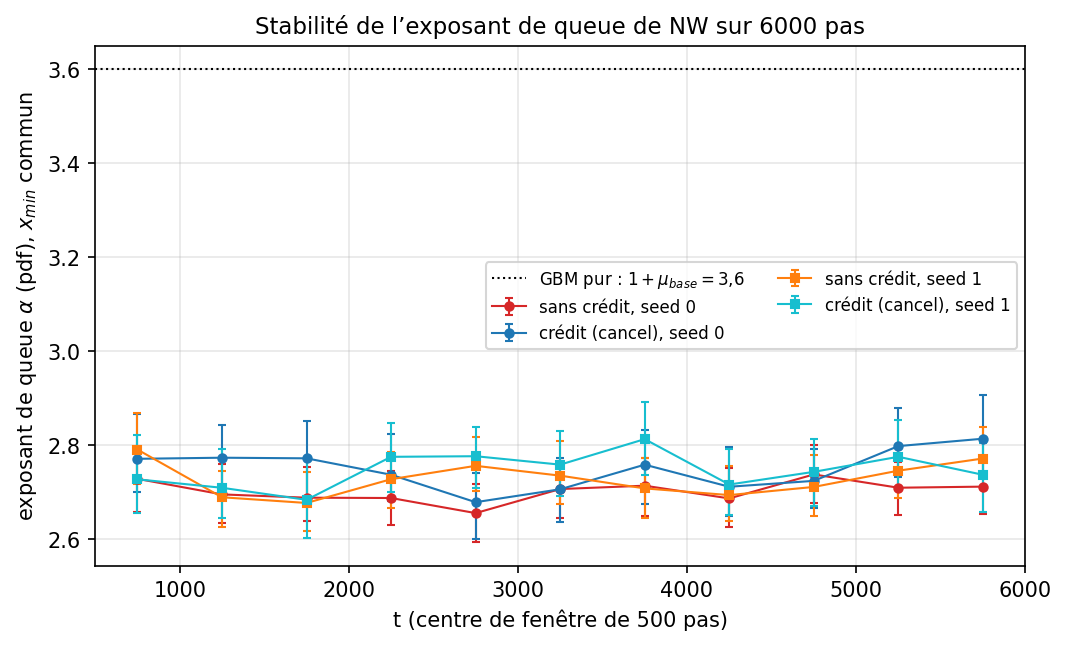
\includegraphics[width=0.88\textwidth]{figures/alpha_drift_long.png}
\end{center}
\noindent Exposant de queue de $\NW$ par fenêtres de 500 pas sur
$T = 6000$, à $x_{\min}$ commun, IC bootstrap 95\,\%. Les runs \emph{sans
aucun crédit} (rouge/orange) sont indiscernables des runs avec crédit
(bleu/cyan) : même exposant, même stabilité, loin du repère GBM--Kesten pur
(pointillés, $\alpha = 3{,}6$) — c'est le mélange démographique (âges
exponentiels $\times$ trajectoires log-normales tuées au plancher) qui fixe
et stabilise l'exposant. Corollaire : \textbf{la stabilité observée ne
valide pas H2}, elle est acquise sans elle.

\section{Trois artefacts débusqués (et corrigés)}
\begin{enumerate}[leftmargin=1.6em, itemsep=4pt]
\item \textbf{Le test « loi de puissance vs log-normale » était truqué —
  involontairement.} Le script hérité \code{tail\_test.py} conclut
  « Pareto, $p \approx 0$ » \emph{même sur des données log-normales pures}
  ($R = +575$ ; les logs [E7c] : $+566$ à $+694$…). Cause : log-normale de
  comparaison non renormalisée par la troncature en $x_{\min}$. Avec le LR
  corrigé (MLE tronqué), le verdict s'inverse dans les 31 fenêtres sur 31 :
  \textbf{la preuve de queue de Pareto du rapport de conception était un
  artefact d'outillage}.
\item \textbf{Le critère AIC du corps était biaisé contre l'exponentielle} :
  ajuster des familles non tronquées sur les 95\,\% inférieurs fait perdre
  la vraie famille ($\Delta$AIC $= 31$ contre une exponentielle pure). Le
  MLE tronqué corrige ; le verdict « corps non exponentiel » survit, mais
  c'était une chance, pas une garantie de la méthode.
\item \textbf{La règle de faillite M2 fait exploser le carnet de contrats} :
  la scission au prorata est combinatoire — $1244 \to 43\,977$ contrats
  entre $t = 1000$ et $2000$ en baseline, jusqu'à $12{,}4$ \emph{millions}
  sur une case de la grille (30 minutes de calcul pour 6000 entités !). Le
  prototype [E7c] annulait ces contrats : l'écart spec/prototype, non
  documenté, masquait le vice. Correctif validé : fusion des contrats par
  paire au taux moyen pondéré (variante \code{merge\_pairs}, flux
  rigoureusement préservés, carnet borné).
\end{enumerate}

\section{Découvertes de robustesse}
\begin{itemize}[leftmargin=1.4em, itemsep=3pt]
\item \textbf{La moyenne géométrique des taux est constitutive} : en moyenne
  arithmétique, le marché meurt (176 prêts en 2000 pas, tous mort-nés). Ce
  que le rapport classait « convention à figer, pas à régler » est en
  réalité la condition d'existence du crédit.
\item \textbf{La fenêtre de naissance est binaire} : à $\sigma = 0{,}15$, la
  mortalité s'éteint et la population diverge (15--20k) ; à
  $\sigma = 0{,}35$, $N^* \approx 200$--$450$. La forme est robuste
  \emph{dans} la fenêtre ; l'existence du régime ne l'est pas.
\item \textbf{Réponse de l'exposant à $\sigma$} : $3{,}8 \to 2{,}7 \to
  2{,}2$--$2{,}4$ pour $\sigma = 0{,}15/0{,}25/0{,}35$ — monotone et lisse ;
  quasi insensible à $\varepsilon_0/w_0$ (0,05--0,5) et à $k$ (2--6).
\item \textbf{La condensation par prorata n'est pas le moteur de la queue}
  (variante \code{destroy} identique) — notre principale hypothèse
  alternative est réfutée, au crédit du modèle.
\item \textbf{Personne ne meurt riche} : la mortalité instantanée du top
  décile est nulle ; on descend d'abord, on meurt pauvre. Le critère
  « mortalité du top $> 0$ » du rapport était mal posé ; le renouvellement
  (90--95\,\%) est la bonne mesure.
\end{itemize}

\section{Réponses expresses au cahier des charges}
\renewcommand{\arraystretch}{1.35}
\begin{center}
\small
\begin{tabular}{p{7.2cm}p{7.6cm}}
\toprule
\textbf{Question} & \textbf{Réponse} \\
\midrule
Implémentation fidèle ? & Oui (spec §2.2 + conventions C1--C10 documentées) ;
le prototype du rapport, lui, ne l'était pas. \\
Corps exponentiel ? & Non au sens statistique (Fisk) ; quasi, en pratique,
pour $\NW$ à $\sigma = 0{,}25$ ; franchement non pour le revenu
($\mathrm{med}/\mathrm{mean} = 0{,}92$). \\
Queue de Pareto stable ? & Exposant effectif très stable (6000 pas) ; mais
log-normale tronquée préférée partout, et le crédit n'y contribue pas. \\
Classes dynamiques ou démographiques ? & Dynamiques, sans ambiguïté. \\
Population bornée endogènement ? & Oui, dans la fenêtre de naissance — et
même sans crédit. \\
Robuste sans réglage fin ? & La \emph{forme} oui (dans la fenêtre) ; le
\emph{régime} exige la fenêtre ; deux conventions sont porteuses. \\
\bottomrule
\end{tabular}
\end{center}

\section{Et maintenant ?}
\begin{enumerate}[leftmargin=1.6em, itemsep=3pt]
\item \textbf{Chercher un régime où le crédit compte} : marché plus dense,
  chocs corrélés entre entités (le choc i.i.d. moyenne le risque de
  portefeuille et étouffe les cascades), $\lambda$ faible (laisser la place
  au canal financier), taux plus élevés sans tuer le marché.
\item \textbf{Théorie du corps Fisk} : dériver la loi stationnaire du
  processus individuel (GBM $+$ $\sqrt{w} - \delta w$, tué à $\NW = 0$,
  réinjecté à $\varepsilon_0$) ; expliquer la coïncidence
  $\mathrm{med}/\mathrm{mean} \approx \ln 2$ à $\sigma = 0{,}25$.
\item Invariance d'échelle de temps ($\delta \to \delta/2$), grille à 3
  seeds, consolidation par paire par défaut si le prorata est conservé.
\end{enumerate}

\begin{encadre}[nonrouge]{À retenir pour la suite du programme de recherche}
Le triplet \{choc $\sigma$, extraction$-$dépréciation, plancher $d_0$ +
naissances Poisson\} est un \emph{excellent} générateur minimal de
distribution stationnaire quasi-Boltzmann--Pareto — c'est un résultat
positif et exploitable. Mais la charge de la preuve est désormais inversée :
c'est à la thèse SOC d'exhiber un régime où le crédit produit un effet
distributionnel détectable, faute de quoi M2 doit être re-décrit pour ce
qu'il est — un modèle démographique de renouvellement, habillé d'un marché.
\end{encadre}

\end{document}
